\documentclass{article}

% if you need to pass options to natbib, use, e.g.:
%     \PassOptionsToPackage{numbers, compress}{natbib}
% before loading neurips_2020

% ready for submission
% \usepackage{neurips_2020}

% to compile a preprint version, e.g., for submission to arXiv, add add the
% [preprint] option:
    % \usepackage[preprint,nonatbib]{neurips_2020}

% to compile a camera-ready version, add the [final] option, e.g.:
    \usepackage[final]{neurips_2020}

% to avoid loading the natbib package, add option nonatbib:
    %  \usepackage[nonatbib]{neurips_2020}

\usepackage{graphics}
\usepackage{textcomp}
\usepackage{graphicx}
\usepackage{wrapfig}
\usepackage{amsfonts}
\usepackage{algorithm,algorithmicx}
\usepackage{algpseudocode}
\usepackage{microtype}      % microtypography
\usepackage{pdfpages}
\usepackage{amsmath}
\usepackage{amssymb}
\usepackage{float}
\usepackage{amsthm}
\usepackage{multicol}
\usepackage[toc,page]{appendix}
\usepackage{balance} % for balancing columns on the final page
\usepackage{caption} 
\usepackage{hyperref}
\hypersetup{
    colorlinks=true,
    linkcolor=blue,
    urlcolor=blue,
    citecolor=blue
}

\newtheorem{innercustomgeneric}{\customgenericname}
\providecommand{\customgenericname}{}
\newcommand{\newcustomtheorem}[2]{%
  \newenvironment{#1}[1]
  {%
   \renewcommand\customgenericname{#2}%
   \renewcommand\theinnercustomgeneric{##1}%
   \innercustomgeneric
  }
  {\endinnercustomgeneric}
}

\newcustomtheorem{customthm}{Theorem}
\newcustomtheorem{customlemma}{Lemma}

\title{On Variational Generalization Bounds for Unsupervised Visual Recognition}

% The \author macro works with any number of authors. There are two commands
% used to separate the names and addresses of multiple authors: \And and \AND.
%
% Using \And between authors leaves it to LaTeX to determine where to break the
% lines. Using \AND forces a line break at that point. So, if LaTeX puts 3 of 4
% authors names on the first line, and the last on the second line, try using
% \AND instead of \And before the third author name.

\author{
  Karush Suri$^{1}$, Mahdi Haghifam$^{1,2}$, Ashish Khisti$^{1}$\\
   $^{1}$University of Toronto, $^{2}$Vector Institute\\
  \texttt{karush.suri@mail.utoronto.ca}
}


\begin{document}

\maketitle

\begin{abstract}
Recent advancements in generalization bounds have led to the development of tight information theoretic and data-dependent measures. Although generalization bounds reduce bias in estimates, they often suffer from tractability during empirical evaluation. The lack of a uniform criterion for estimation of Mutual Information (MI) and selection of divergence measures in conventional bounds hinders utility to sparse distributions. To that end, we revisit generalization through the lens of variational bounds. We identify hindrances based on bias, variance and learning dynamics which prevent accurate approximations of data distributions. Our empirical evaluation carried out on large-scale unsupervised visual recognition tasks highlights the necessity for variational bounds as generalization objectives for learning complex data distributions. Approximated estimates demonstrate low variance and improved convergence in comparison to conventional generalization bounds. Lastly, based on observed hindrances, we propose a theoretical alternative which aims to improve learning and tightness of variational generalization bounds. The proposed approach is motivated by contraction theory and yields a lower bound on MI.   
\end{abstract}

\section{Introduction}
Generalization bounds provide tight measures which facilitate the learning of distributions under sparse data. The work of Russo et. al. \cite{russo} has led to drastic improvements \cite{xu,negrea} in bounding generalization error with information theoretic metrics. The surge of information theoretic metrics \cite{xu,bu} has further motivated improvements in bias reduction for control measurements \cite{cotnrol}. While generalization bounds tighten the dynamics of sparse learning, a tighter approximation often hurts the performance in the presence of out-of distribution samples \cite{mine}. In many such scenarios, it is difficult to empirically evaluate the performance of the bound \cite{control}. Additionally, the abundance of divergence metrics does not provide a selection criterion for an optimal information theoretic entity \cite{book, measures}. This allows one to rethink the feasibility of conventional bounds in practical scenarios. 

Variational bounds \cite{variational} are a class of probabilistic bounds which depict increasing potential for learning \cite{mine,visual,cpc}. A typical variational bound utilizes a tractable data distribution which can be approximated with limited data samples. This property of variational measures motivates data-efficient learning \cite{cpcv2}. Tractibility of variational bounds for information maximization and minimization allows multiple objective functions to be realisable in a given problem setting \cite{variational}. Variational bounds can then be flexibly modeled as lower and upper bounding measures of information \cite{variational}. However, large-scale utilization of multi-sample variational bounds is an open problem for unsupervised learning tasks \cite{variational}. Data-efficient learning in conjunction with tractable compatibility to data distributions presents variational bounds as suitable candidates for learning objective functions.

We revisit the regime of generalization bounds from the perspective of information theoretic and variational distributions. The work highlights the suitability of variational bounds in comparison to conventional generalization bounds which emphasize only on the bias in data estimates. Variational objectives tackle high bias as well as high variance estimates. Our main contributions are threefold- 

\begin{itemize}
    \item We revisit generalization in light of variational learning and identify hindrances which prevent accurate  approximations of data distributions.
    \item We empirically demonstrate the suitability of variational generalization bounds on unsupervised visual recognition tasks wherein the data distribution is inherently challenging to approximate.  Our evaluation highlights the necessity for variational generalization bounds.
    \item We conjecture a theoretical alternative which aims to address the hindrances discovered in learning variational generalization bounds. The proposed approach is motivated by contraction theory and yields a lower bound on MI. 
  \end{itemize}



\section{Related Work}
\textbf{Variational Bounds}: A number of methods \cite{variational,mine,infomax,cpc,cpcv2} introduce variational bounds for information-based learning. MINE \cite{mine} presents the estimation of MI utilizing gradient descent for high-dimensional random variables. Suitability of MINE leads to improved adversarial generative models and supervised classification tasks. InfoMAX \cite{infomax}, extends the MI framework by simultaneously estimating and maximizing information between output representations and input prior distributions. InfoMAX scales well to unsupervised learning scenarios and sparse latent distributions. While, MINE and InfoMAX highlight the practical utility of information estimation, they do so at the cost of large data requirements from the input distribution. CPC \cite{cpc} and CPCv2 \cite{cpcv2} aid data-efficient learning by introducing the InfoNCE bound. The InfoNCE objective eliminates the need for explicit estimation of MI by providing a lower bound on MI. InfoNCE being a multi-sample bound \cite{variational}, scales well in the number of data samples in-distribution. However, the objective is hindered by large batch sizes and is not tight for large values of MI. The recently proposed interpolation bounds \cite{variational} extend the InfoNCE setup towards a continuum of bounds which trade-off bias with variance. Additionally, the bound is tight for varying batch sizes. Our work is orthogonal to the proposed interpolation scheme and extends it to the generalization setup.  

\textbf{Generalization Bounds}: The pivotal work of \cite{russo} provides a lower-bound on MI based on information-theoretic measures \cite{dv,book}. The MI bound \cite{overfit} is further improved as a result of tight lower bounds on MI minimizing the generalization error \cite{xu,bu}. Additional measures such as data-dependent estimates \cite{negrea} and the specific choice of distributions \cite{kuzborskij} extend the application of lower bounds to stochastic learning dynamics \cite{bu,sgld} and differential privacy \cite{russo,zu}. The bounds are further sharpened using conditional MI \cite{haghifam} in a sample-based framework \cite{steinke} which extends the data-dependent scheme of \cite{negrea}. A more suitable application is the setting of adaptive control \cite{control} which is based on high stochasticity stemming from continuous measurements. The bound provided in \cite{control} aims to address this problem with the introduction of $alpha$ divergence metrics \cite{measures} which serve as a lower bound on MI. While the bound is proven to be theoretically tight, its application and empirical evaluation remain an open problem in literature. We aim to leverage the theoretical contributions of \cite{control} in order to provide a variational alternative which can be empirically realised.

\textbf{Unsupervised Visual Recognition}: One of the main applications of information-theoretic bounds is unsupervised learning for visual recognition tasks \cite{visual}. The information maximization framework \cite{infomax} reduces local sparsity and motivates the learning of richer representations \cite{cpc}. Multi-sample bounds such as InfoNCE in CPC \cite{cpc} and CPCv2 \cite{cpcv2} contrast augmented representations with actual input samples in order to maximize MI among local pixels. MOCO \cite{moco,mocov2} extends the setup of InfoNCE further with the pretext contrast as a dictionary-lookup task. InfoNCE bound is combined with a momentum encoder which maximizes MI as a slow moving average of input and augmented samples. SimCLR \cite{simclr} builds on the MOCO framework by maximizing the internal agreement between representations. While unsupervised representation learning methods adopt lower bounds on MI, they do so at the cost of large batch sizes. Since the InfoNCE bound is lose at small batch sizes, large architectures lean towards pretraining alternatives \cite{simclrv2} rather than improving lower bounds. The work of \cite{visual} adapts InfoNCE bound based on parameteric and non-parameteric learning of visual instance discrimination. The multi-sample classification is casted to a binary discrimination setup, hence providing improved generalization and consistent performance. Based on this insight, we adopt the instance discrimination setup of \cite{visual} for our experiments. 

\section{Preliminaries}
We review the information-theoretic setup for generalization and variational bounds. Let $X$ and $Y$ be a pair of random variables denoting the input and output data distributions $p(x)$ and $p(y)$ respectively. The mutual information $I(X;Y)$ between $X$ and $Y$ is a reparameterization-invariant measure of dependency consisting of the joint distribution $p(x,y)$and can be mathematically expressed as follows,
\begin{gather}
  I(X;Y) = \mathbb{E}_{p(x,y)}[\log\frac{p(x|y)}{p(x)}] = \mathbb{E}_{p(x,y)}[\log\frac{p(y|x)}{p(y)}] \label{eq:inf}
\end{gather}
\autoref{eq:inf} can be further simplified by exapnding the expectation, 
\begin{gather}
  I(X;Y) = \sum_{y}p(x|y)p(y)\log\frac{p(x|y)}{p(x)} = \mathbb{E}_{p(y)}[D_{KL}(p(x|y)||p(x))] \label{eq:infsimp}
\end{gather}
$D_{KL}$ in \autoref{eq:infsimp} denotes the Kullback-Liebler (KL) Divergence \cite{kl} which is a divergence metric. $D_{KL}$ belongs to the general class of $\phi-$divergence metrics $D_{\phi}(P(x)||Q(y))$ which quantify the similarity between any two data distributions $P(x)$ and $Q(y)$. The general form of a $\phi$-divergence, with $\phi$ being a convex and lower semi-continuous function such that $\phi(1)=0$, is expressed in \autoref{eq:phi}. Utilizing $\phi(t)=t\log t$ in \autoref{eq:phi} yields $D_{\phi}(P(x)||Q(y))=D_{KL}(P(x)||Q(y))$.
\begin{gather}
  D_{\phi}(P(x)||Q(y)) = \sum_{y}Q(y)\phi(\frac{P(x)}{Q(y)}) \label{eq:phi}
\end{gather}   
Generalization bounds make use of random variables with a cumulant-generation \cite{cover} function $\psi(\lambda) = \log\mathbb{E}[e^{\lambda x}]$ such that $\lambda \geq 0$. A random variable is called $\sigma$-sub-Gaussian if the argument of the $\log$ cumulant-generation function satisfies $\mathbb{E}[e^{\lambda x}] \leq e^{\frac{\lambda^{2}}\sigma^{2}}{2}$ for all $\lambda \in \mathbb{R}$ with $\sigma^{2}$ as the variance proxy or variance factor of the distribution.  
% all background with notations


\section{When Do Bounds Hurt Learning?}
% explain the problems here, demonstrate using table with tick marks and crosses, provide a visual (of distribution) as well, cite examples and mathematical flaws
The work of \cite{variational} throws light on the behavior of tractable distributions with high dimensional random variables. Based on the empirical characteristics of these bounds, one can identify the hindrances faced in generalization of the leanring algorithm (see \autoref{fig:dist}).

\textbf{High Variance}: Normalized upper and lower bounds aid in tractability of variational distributions when the data to be learned is long-tailed. However, these bounds demonstrate high variance as a result of large MI estimates. A suitable alternative to normalized bounds is to adopt the framework of structured bounds. These bounds leverage the structure of the problem and yield a known conditional distribution $p(y|x)$ which is tractable as per the problem setting. Structured bounds are conveniently applicable to representation learning \cite{cpc,variational} but do not necessarily scale to high-dimensional scenarios. Another alternative which provisions a conitional tractable distribution are reparameterization bounds. These bounds make use of an additional functional, known as the \textit{critic}, which converts lower bounds on MI into upper bounds on KL divergence. The critic functional need not explicitly learn the mapping between $x$ and $y$. However, reparameterization is only made feasible if the conditional distribution $p(y|x)$ is tractable. 

\textbf{High Bias}: Unnormalized upper and lower bounds demonstrate high bias and hurt tractability of complex distributions. Primary reasons for instability in bounds is lack of a partition functional which normalizes MI estimates. \cite{variational} argues that requirement of a partition function presents high bias as a result of exponential distributions which may not be tractable. However, the work does not provide empirical evidence on their tractability which leaves the suitability of a normalization constant an pen question. A suitable alternative to address biased estimates is the adoption of density ratios which train the critic functional using a divergence metric. The Jensen-Shanon Divergence (JSD) is one such scheme which yields a lower-biased estimate of optimal critic. While training critics is theoretically suitable, empirical evaluations \cite{variational} demonstrate unstable convergence of exponential gradients. 

\begin{figure*}[ht]
  \centering
  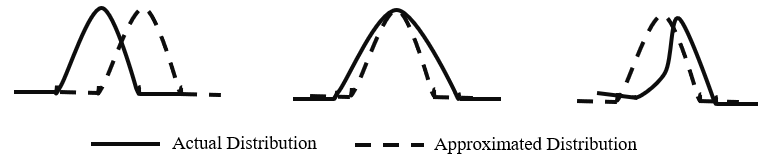
\includegraphics[height=2.5cm,width=13cm]{dist.PNG}
  \caption{\textbf{Left} Conventional lose bounds suffer from high bias which hurts generalization of the learnt distribution, \textbf{Center} Learnt distribution is additionally hampered with noisy approximations, \textbf{Right} Biased estimates in conjunction with noisy dynamics hurt the completeness of learnt data distributions.}
  \label{fig:dist}
\end{figure*}

\textbf{A Failure to Learn}:  Multi-sample bounds proposed in conjunction with $\alpha$-MI saturates at $\log K$ with $K$ being the number of samples in the batch. 

% demonstrate DV empirically and highlight its consequences
% highlight the importance of alpha I and difficulty in selection of optimal alpha

\section{Variational Bounds for Generalization}
% explain what the section is about and what you wish to accomplish, make sure to be mathematical

\subsection{Learning Variational Bounds}
% review the bounds here, critically comment on their usage

\subsection{Bias Reduction as Contraction}
% provide your novelty, explain its usage well
% maybe use extreme value theory to prove the tightness of InfoNCE
% maybe combine InfoNCE with control bound

\section{Experiments}
% state your objectives and what you wish to assess
\subsection{Setup}
% explain the setup 

\subsection{Unsupervised Instant Discrimination}
% provide tabular results, emphasize on whay and how

\section{Conclusion}

\bibliographystyle{unsrt} 
\small{\bibliography{sample}}

% 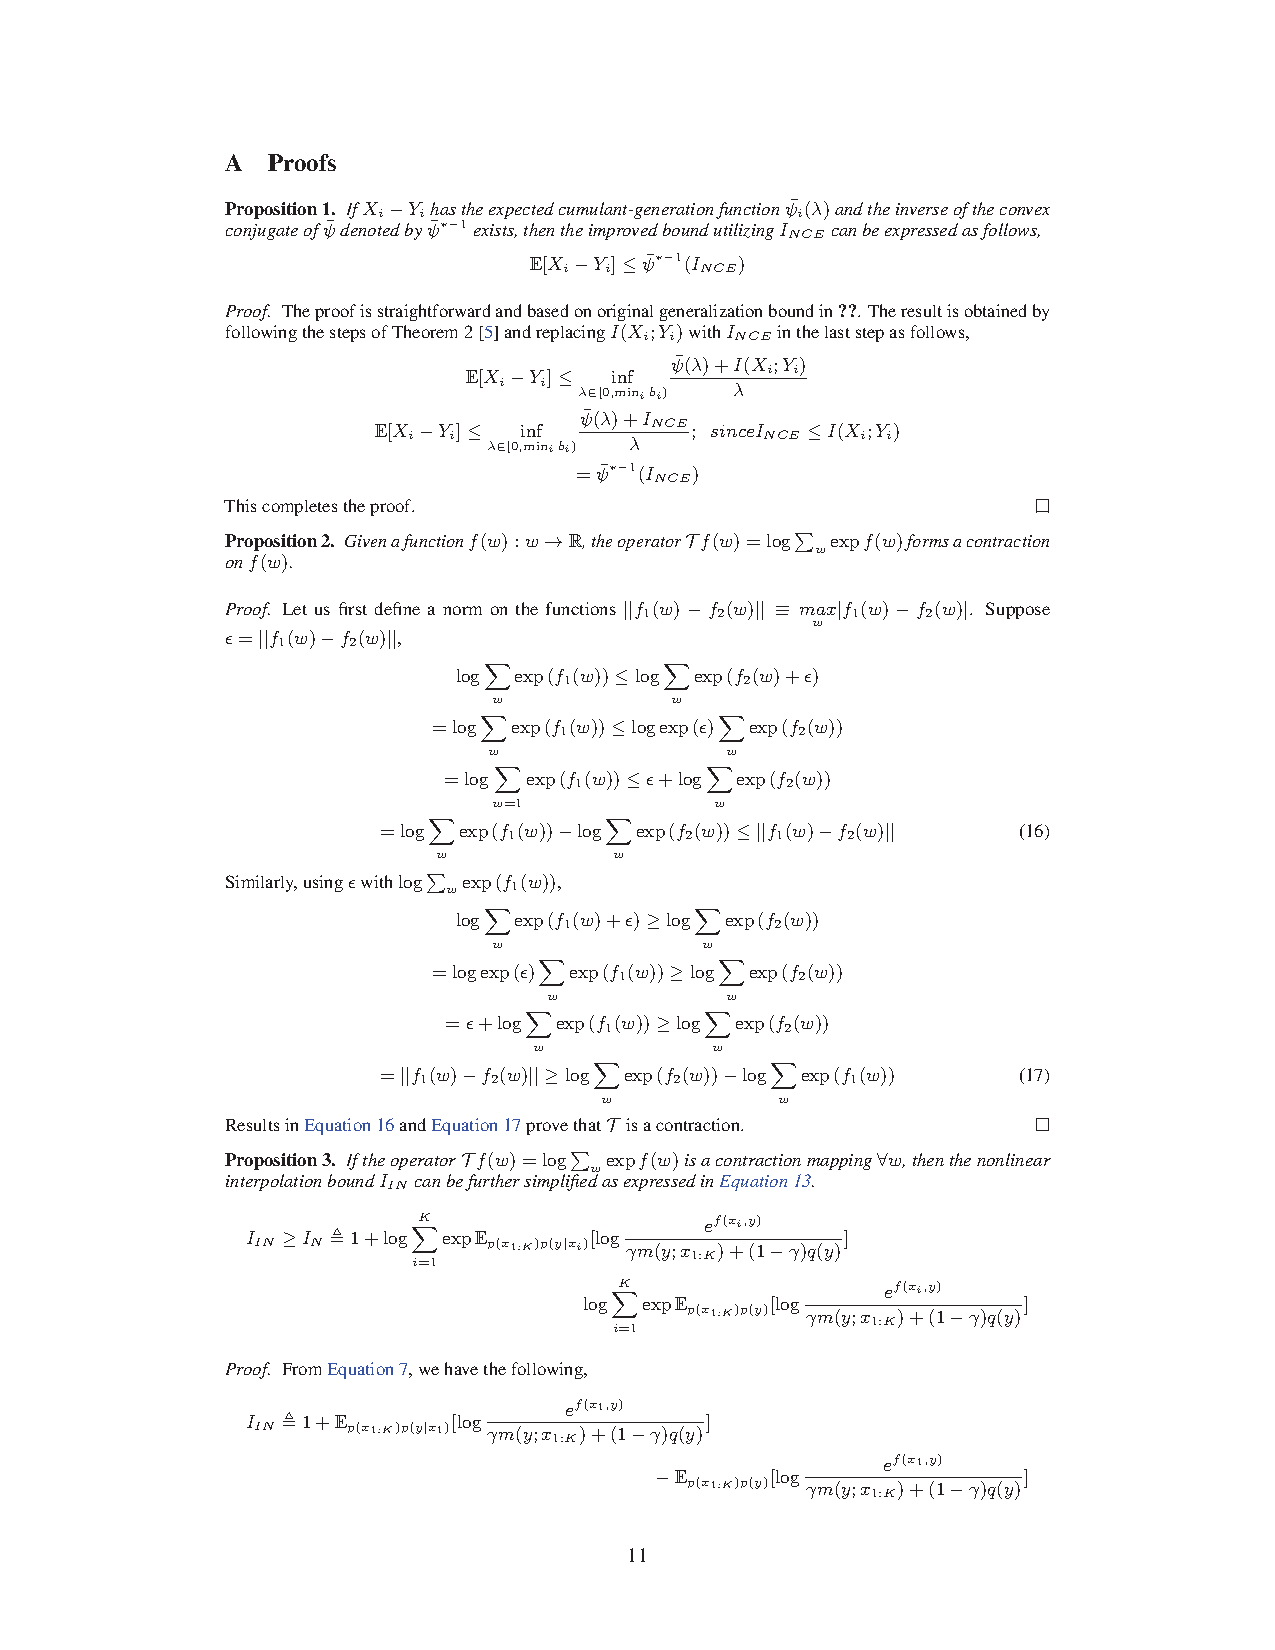
\includepdf[pages=-]{Appendix}


\end{document}
